
\documentclass[12pt]{article}
\usepackage[utf8]{inputenc}

\usepackage[a4paper, margin=1in]{geometry}

\usepackage{newtxtext}
\usepackage{amsmath,amssymb,amsthm}
\usepackage{newtxmath} % must come after amsXXX

\usepackage{float}%防止图片乱跑



\usepackage{graphicx}
%\usepackage{subfigure}




\usepackage{xcolor}
\usepackage{fancyhdr}

\usepackage{listings}
%\usepackage{ctex}

\usepackage{booktabs}


%%%%%%%%%%%% for sudocode %%%%%%%
\usepackage{algorithm}
\usepackage{algpseudocode}
%%%%%%%%%%%%%%%%%%%%%%%%%%%%%%%%%





%%%%%%%%%%%%%%%%%%%%%%%%%%%%%%%%%%%%%%%%%%%%%%%%%%%%%%%%%%%%%%%
%%%%%%%%%%%%%%%%%%%%%%%%%%%%%%%%%%%%%%%%%%%%%%%%%%%%%%%%%%%%%%%

\begin{document}

\title{EN 530.766\\Fall 2023\\HW 4–Haobo Zhao}
\maketitle

\begin{abstract}
    This report is an approach using 2D-Finite Difference method to
    simulate the Elliptic problem (Jacobi, Gauss-Seidel, SOR, SRJ),
    as the boundary condition, grid, 
    and control equation are provided.

    In the first question, use Jacobi iteration method and Gauss-Seidel
    (G-S) method to iterate, and calculated the residual and the
    iteration error (absolute sum of residual). It could be found that 
    the error is droping fast as the iteration number 
    growing, initial guess (IG)=0 converge fastest among IGs, G-S method is  
    converge faster than Jacobi except for IG=0.
    
    For the question (2), by use SOR point Jacobi and 
    SOR point G-S method, introducing relaxization parameter w, 
    found optimal w is around 1.7 for G-S method according all IG. But 
    still, w=1 is best for Jacobi.

    For the third question, use the SRJ method, alternatively using w1 and w2,
    where w1 for underrelaxation and w2 for overrelaxation, found the best
    combination for w1 and w2 is (0.7,2.0), while frequency (1:1).

    For the question (4), by choose and compare different groups of
    w1, w2, and w3, found the optimal (w1,w2,w3) group: (9.3,1.1,1.0) for 
    frequency (1:9:90), converge faster than non-relaxed Jacobi, and 
    2-parameter SRJ, which means is still possible to try more parameters or
    wide range of frequency combination



\end{abstract}



\tableofcontents











%%%%%%%%%%%%%%%%%%%%%%%%%%%%%%%%%%%%%%%%%%%%%%%%%%%%%%%%%%%%%%%
%%%%%%%%%%%%%%%%%%%%%%%%%%%%%%%%%%%%%%%%%%%%%%%%%%%%%%%%%%%%%%%

\section{Review of Questions}




\noindent Consider the 2-D Laplace equation
\begin{equation*}
    (u_{xx} + u_{yy}) = 0 \quad \text{for } 0 < x,y < 2\pi
\end{equation*}
with the following boundary conditions
\begin{align*}
    u(0,y) &= 0 \\
    u(2\pi,y) &= 0 \\
    u(x,0) &= \sin(2x) + \sin(5x) + \sin(7x) \\
    u(x,2\pi) &= 0
\end{align*}

\begin{enumerate}
    \item Write a computer code and obtain the numerical solution 
    using the point Jacobi and Gauss-Seidel iterative schemes. Use 
    a mesh with $\Delta x = \Delta y = \frac{2\pi}{20}$. Track the 
    convergence by calculating the residual, 
    $r^k = (\frac{\delta_{x}^2}{\Delta x^2} + \frac{\delta_{y}^2}{\Delta y^2} ) u_{i,j}^k$
    
    Conduct these simulation with two different initial guesses 

    (1) $u(i,j) = 0$; 

    (2) $u(i,j) = {x_i}y_j$

    (3) $u(i,j) = \text{random number distribution between -1 and 1.}$

    Does the convergence behave as expected? Discuss.

    \item Try the above problem with the SOR point Jacobi and 
    SOR point Gauss-Seidel schemes: Investigate and comment on 
    the convergence properties for various values of the under- 
    and over-relaxation parameter for both schemes. Can you find 
    optimal values of the relaxation parameter for these schemes?

    \item Experiment with a SOR Jacobi method where you alternate 
    between an overrelaxation and an underrelaxation as you iterate. 
    Can you find a pair of relaxation parameters that speed up the 
    solution process compared to the non-relaxed Jacobi method? For 
    more information about this ``Scheduled Relaxation Jacobi'' Method 
    check out this paper: \textit{Xiang Yang and Rajat Mittal, ``Acceleration 
    of the Jacobi iterative method by factors exceeding 100 using 
    scheduled relaxation'', Journal of Computational Physics, Vol 274, 
    DOI: 10.1016/j.jcp.2014.06.010.}

    \item Challenge problem – how about experimentally determining 
    a SRJ scheme with 3 different values of the relaxation parameter.
     How much faster can you get compared to the 2 parameter SRJ scheme.
\end{enumerate}



%%%%%%%%%%%%%%%%%%%%%%%%%%%%%%%%%%%%%%%%%%%%%%%%%%%%%%%%%%%%%%%
%%%%%%%%%%%%%%%%%%%%%%%%%%%%%%%%%%%%%%%%%%%%%%%%%%%%%%%%%%%%%%%



\section{(1): Simulation, resudual compare}
%%%%%%%%%%%%%%%%%%%%%%%%%%%%%%%%%%%%%%%%%%%%%%%%%%%%%%%%%%%%%%%
\subsection{Jacobi, Gauss-Seidel Iteration, Residual}
For problem 1, use sudo-time, let Jacobi and Gauss-Seidel iteration 
method to obtain the next iteration solution. Compare the solution 
with the Elliptic source term, could occour residual, and take absolute
value sum of residual to get total error, as the index of each
method's performance.\\

The steps of the approach is showing below:

The control equation is showing below:

\begin{equation*}
    (u_{xx} + u_{yy}) = 0 \quad \text{for } 0 < x,y < 2\pi
\end{equation*}

Or in other notation: $$\nabla^2 P = 0 \quad $$


Add sudo-time part, obtain:
$$\nabla^2 P = \frac{\partial P}{\partial t}$$


Where is also can be shown as: 
\begin{equation*}
    (u_{xx} + u_{yy}) = u_{t} \quad \text{for } 0 < x,y < 2\pi\\
\end{equation*}

Transfer Partial Difference Equartion (PDE) to Finite Difference equation
(FDE), use central difference method for spacial derivative transform, and
use forward difference for ``time" transformk, obtained:

\begin{align*}
    \frac{P_{ij}^{k+1} - P_{ij}^k}{\Delta t} &= \frac{1}{\Delta^2} \left[ P_{i-1,j}^k + P_{i+1,j}^k + P_{i,j-1}^k + P_{i,j+1}^k - 4P_{ij}^k \right]
\end{align*}

For stability, in 1-D scheme, r =<1/2, in 2-D scheme, r =< 1/4.
To obatin the biggest dt, let r= 1/4, which is $\frac{\Delta t}{\Delta^2} = \frac{1}{4}$,
where the FDE transfer to:

\begin{align*}
    \quad P_{ij}^{k+1} &= \frac{1}{4} \left[ P_{i-1,j}^k + P_{i+1,j}^k + P_{i,j-1}^k + P_{i,j+1}^k \right]
\end{align*}

The formula shown above is Jacobi iteration method.
For Gauss Seidel method, the equation is showing below:

\begin{align*}
    \quad P_{ij}^{k+1} &= \frac{1}{4} \left[ P_{i-1,j}^{k+1} + P_{i+1,j}^k + P_{i,j-1}^{k+1} + P_{i,j+1}^k \right]
\end{align*}

For residual, it could be calculated by compare our simulation result with
the source term, which is 0 in this scenario:

\begin{align*}
    r^k &= \frac{1}{\Delta^2} \left[ P_{i-1,j}^k + P_{i+1,j}^k + P_{i,j-1}^k + P_{i,j+1}^k - 4P_{ij}^k \right]
\end{align*}



%%%%%%%%%%%%%%%%%%%%%%%%%%%%%%%%%%%%%%%%%%%%%%%%%%%%%%%%%%%%%%%
\subsection{Algorithms for Jacobi, G-S, and Residual}
Base on this, the Algoritm for Jacobi iteration method can be written:

%%%%%%%%%%%% sudocode %%%%%
\begin{algorithm}
    \caption{Pseudocode for Jacobi Solver}
    \begin{algorithmic}[1]
        \Function{Jacobi}{$P_{\text{input}}, \Delta x, \Delta y, Nx, Ny$}
        \State $P_{\text{old}} \gets P_{\text{input}}$
        \State $P_{\text{new}} \gets P_{\text{input}}$
        \For{$ j=1 $ to $Ny-1$ }
            \For{$ i=1 $ to $Nx-1$ }
                \State $P_{\text{new}}[i][j] \gets \frac{1}{4} (P_{\text{old}}[i-1][j] + P_{\text{old}}[i+1][j]$
                \Statex \hspace{\algorithmicindent}\hspace{\algorithmicindent}\hspace{\algorithmicindent}$+ P_{\text{old}}[i][j-1] + P_{\text{old}}[i][j+1])$
                \State $P_{\text{old}} \gets P_{\text{new}}$
            \EndFor
        \EndFor
        \State \Return $P_{\text{new}}$
        \EndFunction
    \end{algorithmic}
\end{algorithm}


\begin{algorithm}
    \caption{Pseudocode for Gauss-Seidel Solver}
    \begin{algorithmic}[1]
        \Function{Gauss-Seidel}{$P_input, \Delta x, \Delta y, Nx, Ny$}
            \For{$ j=1 $ to $Ny-1$ }
                \For{$ j=1 $ to $Ny-1$ }
                    \State $P_{\text{new}}[i][j]
                    \gets \frac{1}{4} (P_{\text{new}}[i-1][j] + P_{\text{old}}[i+1][j] + P_{\text{new}}[i][j-1] + P_{\text{old}}[i][j+1])$\\
                    $P_{\text{old}} \gets P_{\text{new}}$
                \EndFor
            \EndFor
            \State \Return $P_{\text{new}}$
        \EndFunction

    \end{algorithmic}
\end{algorithm}






The strture of Python program is showing as follows:



\begin{figure}[H]
    \centering
    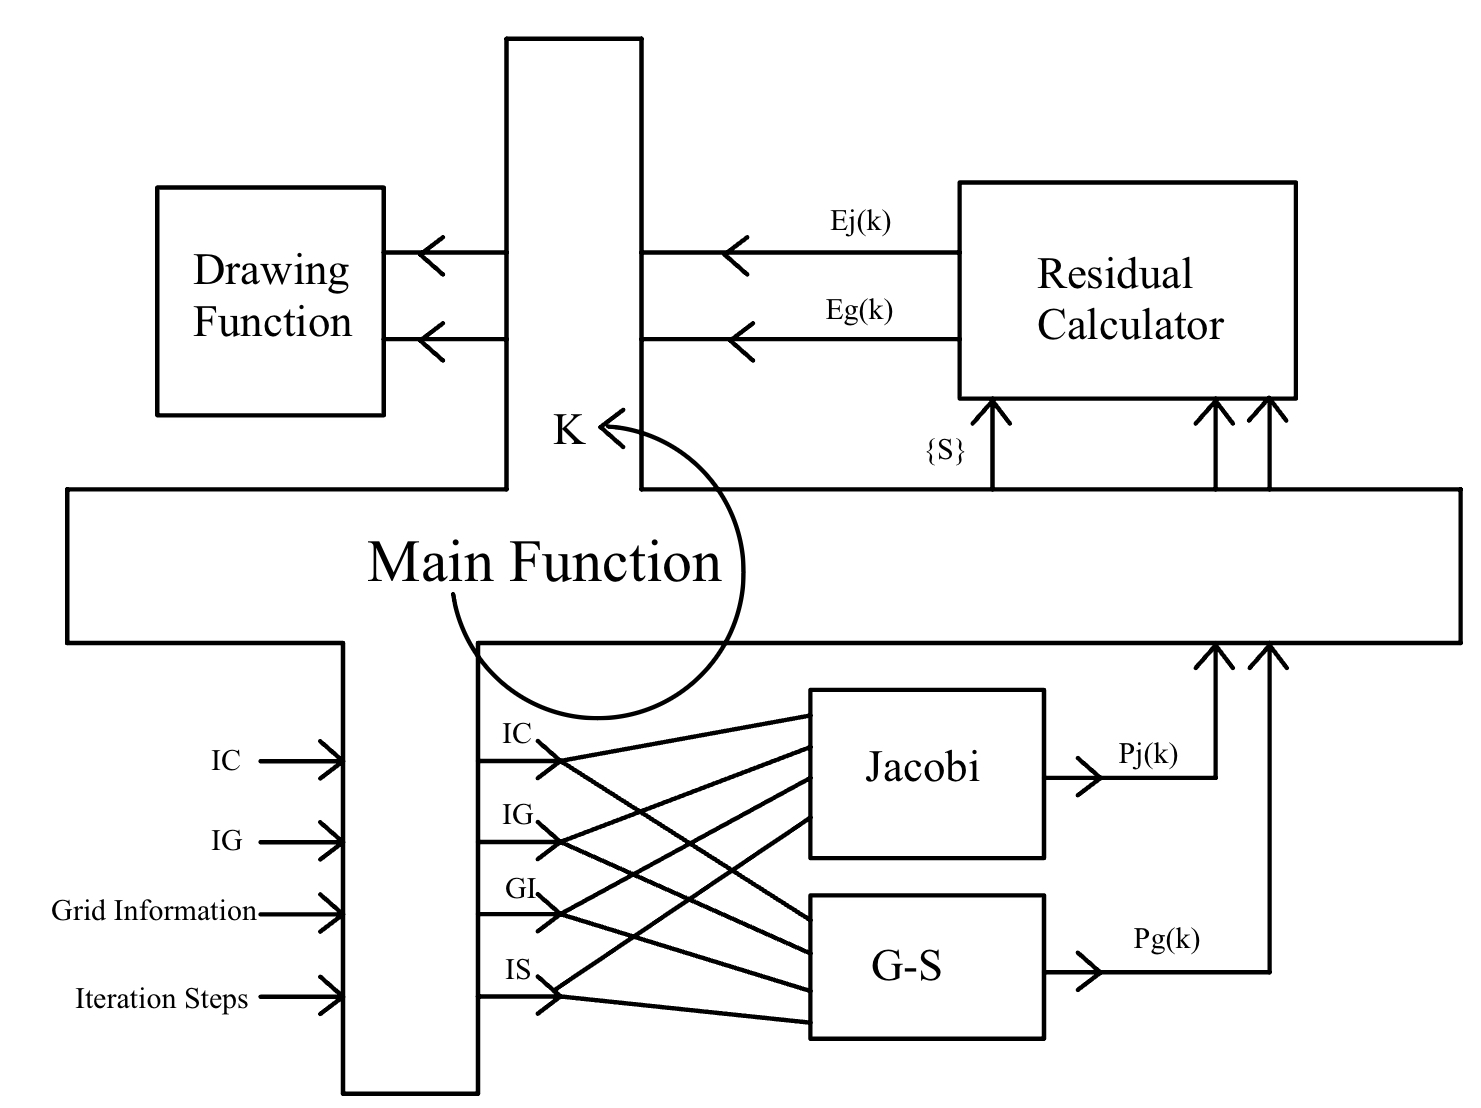
\includegraphics[width=0.6\textwidth]{diagram1.jpg}
    \label{diagram.jpg}
    %\caption{Iteration times as k=200}
\end{figure}



%%%%%%%%%%%%%%%%%%%%%%%%%%%%%%%%%%%%%%%%%%%%%%%%%%%%%%%%%%%%%%%
\subsection{Result and Analysis for (1)}
For iteration(k) 200 times, the result is showing below:


\begin{figure}[H]
    \centering
    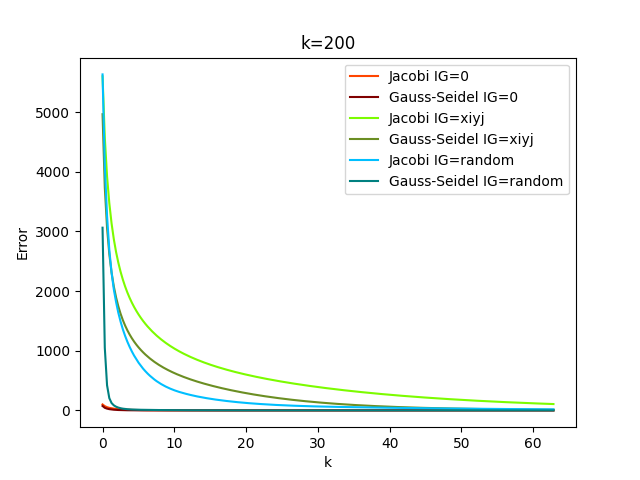
\includegraphics[width=0.7\textwidth]{plotall.jpg}
    \label{plotall.jpg}
    %\caption{Iteration times as k=200}
\end{figure}

It can be observed that the error was very huge, but drop really quick
as iteration keep going. Also, if we running more iteration times, the result should be more
accurate. For k=2000, the result is showing below:

\begin{figure}[H]
    \centering
    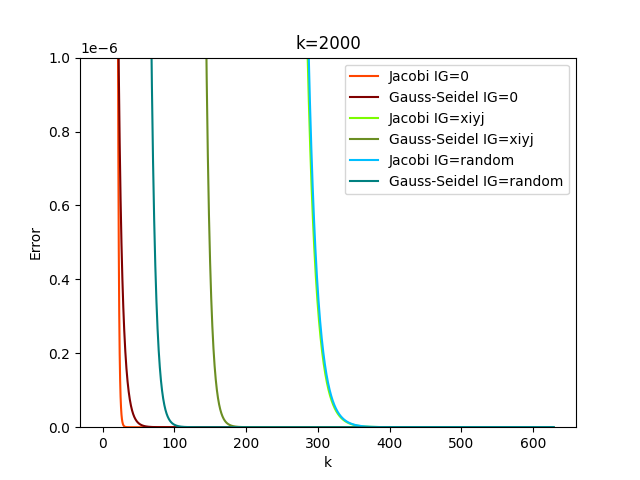
\includegraphics[width=0.8\textwidth]{allIGdetails.png}
    \label{allIGdetails.png}
    %\caption{Iteration times as k=2000, limit y in O($10^{-4}$)}
\end{figure}

The figure arrange different initial guess(IG) in different color set.
For IG=0, Jacobi is the shallow red line, while G-S is in heavy red.
Same as Jacobi and G-S in green with IG=xiyj, and in blue as IG=random.\\


\subsubsection{Analysis For IGs}
Compare different initial condition (IG), it is easily to find that 
IG=0 makes the fastest IG to let error back to 0, while other two are 
pretty close. That may because IG=0 is the closet IG with the actual 
result that boundary condition (3 sides are 0, one side is combination
of sin) created.\\



\subsubsection{Analysis For Jacobi and Gauss-Seidel}

Compare Jacobi and Gauss-seidul (G-S) in each IG, it is can be observed
Gauss-Seidel converge much faster than Jacobi, except for IG=0, where 
Jacobi finally converge faster than Gauss-Seidel.
This could be explained by the wavenumber-analysis:
As the control equation is linear, the wavenumber of result all come from initial guess
(IG) and boundary conditions (BC).\\

\textbf{IG=0}

For IG=0, the wavenumbers are all come from BCs, where k=2,5,7
($u(x,0) = \sin(2x) + \sin(5x) + \sin(7x)$), then $\frac{\beta}{\pi}$= 0.2, 0.5, 0.7.



\begin{figure}[H]
    \centering
    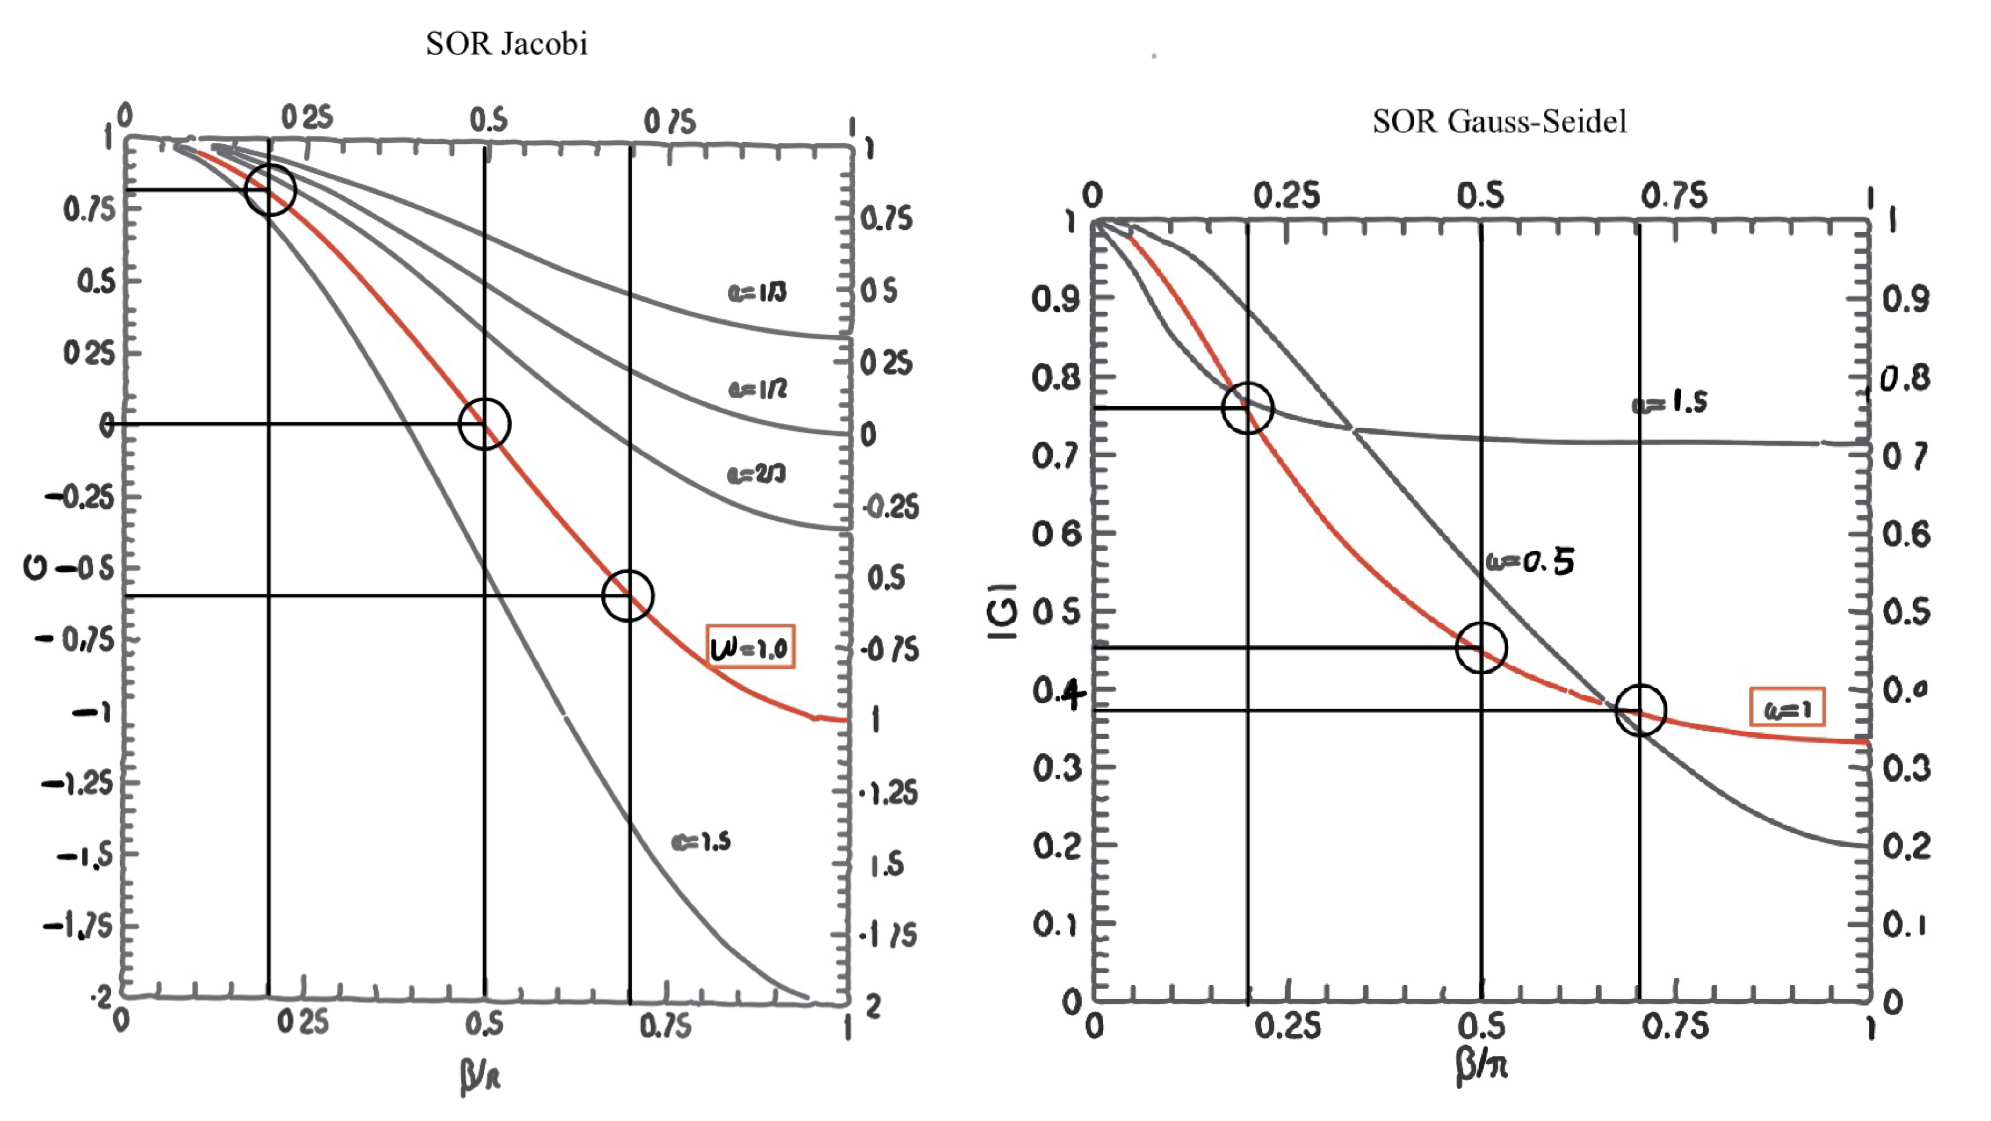
\includegraphics[width=0.8\textwidth]{IGs.jpg}
    \label{IGs.jpg}
    %\caption{Iteration times as k=2000, limit y in O($10^{-4}$)}
\end{figure}


The diagram shows $\frac{\beta}{\pi}$= 0.2, Jacobi and G-S's G are almost same
(G-S is about 0.05 lower than Jacobi),
but for $\frac{\beta}{\pi}$= 0.5, Jacobi's Amplifaction factor(G) is 0, while G-S is 
almost 0.45 (Jacobi is 0.45 lower than G-S).\\

For $\frac{\beta}{\pi}$= 0.7, G(G-S) is 0.28 lower than G(Jacobi).\\


It could be seen that the huge difference in low wave number of Jacobi with
Gauss-Sediel is $\frac{\beta}{\pi}$= 0.5, which could determined the early converge 
rate's difference. However, on $\frac{\beta}{\pi}$= 0.2, G-S Amp factors
is still little bit smaller than Jacobi, which means finally, G-S's error will
smaller than Jacobi, at the same iteration step. Consider this iteration much be
pretty large (the Amp factor on $\frac{\beta}{\pi}$= 0.2's difference is very small), 
and our result, it could consider when it happen, the error will get to the order
of computer round-off error, which means is hard to shown that point where G-S will
finally 'defeat' jacobi.\\

\textbf{IG=xiyj}

For IG=xiyj, it could be seen for fixed one direction, the fourier series of IG can 
be shown as $y = x_{0} \sum_{n=1}^{\infty} \frac{-2(-1)^n L^2}{\pi n L} \sin\left(\frac{n\pi x}{L}\right)$
, where wave number is decreasing among the other direction veryfast: 


\begin{figure}[H]
    \centering
    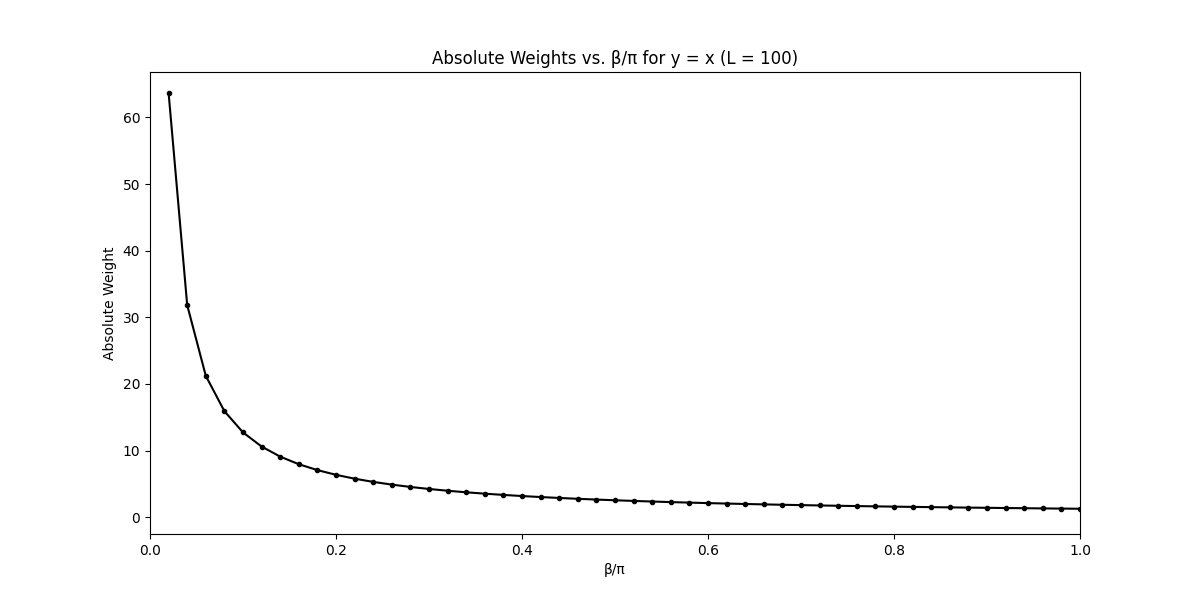
\includegraphics[width=0.8\textwidth]{wavenmubers.png}
    \label{wavenmubers.png}
    %\caption{Iteration times as k=2000, limit y in O($10^{-4}$)}
\end{figure}


It could be seen lowest wavenumebr takes highest weight, where G-S works better
than Jacobi.\\

\textbf{IG=random}

For IG=random, the wavenumebr distribute evenlly among all $\beta$, also according
the diagram before, for most part G-S's error Amplifaction factor is smaller than
Jacobi. Combine the result before, it converge as expected.







\section{(2) SOR Method Approach}
\subsection{SOR Jacobi and SOR Gauss-Sediel}

For the Successive Over-Relaxation (SOR) method, it using w as parameter,
the formula is showing below:


\begin{equation}
    P^{k+1} = (1-\omega)P^{k} + \omega P^*
\end{equation}
    




For SOR Jacobi method, the $P^*$ can be express is as follows:

\begin{equation}
    P^* = \frac{1}{4} \left[ P^{k}_{i-1,j} + P^{k}_{i+1,j} + P^{k}_{i,j-1} + P^{k}_{i,j+1} \right]
\end{equation}

The iteration formula can be shown as:


\begin{equation}
    P^{k+1} = (1-\omega)P^{k} + \frac{\omega}{4} \left[ P^{k}_{i-1,j} + P^{k}_{i+1,j} + P^{k}_{i,j-1} + P^{k}_{i,j+1} \right]
\end{equation}


The algorithm for SOR Solver is showing below:



\begin{algorithm}
    \caption{Pseudocode for SOR Jacobi Solver}
    \begin{algorithmic}[1]
        \Function{Jacobi}{$P_{\text{input}}, \Delta x, \Delta y, Nx, Ny, \omega$}
        \State $P_{\text{old}} \gets P_{\text{input}}$
        \State $P_{\text{new}} \gets P_{\text{input}}$
        \For{$ j=1 $ to $Ny-1$ }
            \For{$ i=1 $ to $Nx-1$ }
                \State $P_{\text{new}}[i][j] \gets 
                (1-\omega)P^{k} + \frac{\omega}{4} \left[ P_{\text{old}}[i-1][j] + P_{\text{old}}[i+1][j] + P_{\text{old}}[i][j-1] + P_{\text{old}}[i][j+1] \right]$
                \State $P_{\text{old}} \gets P_{\text{new}}$
            \EndFor
        \EndFor
        \State \Return $P_{\text{new}}$
        \EndFunction
    \end{algorithmic}
\end{algorithm}




For SOR Gauss-Sediel, $P^*$ is: 


\begin{equation}
    P^* = \frac{1}{4} \left[ P^{k+1}_{i-1,j} + P^{k}_{i+1,j} + P^{k+1}_{i,j-1} + P^{k}_{i,j+1} \right]
\end{equation}


The iteration formula for Gauss-Seidel is showing below:



\begin{equation}
    P^{k+1} = (1-\omega)P^{*} + \frac{\omega}{4} \left[ (P_{\text{new}}[i-1][j] + P_{\text{old}}[i+1][j] + P_{\text{new}}[i][j-1] + P_{\text{old}}[i][j+1]) \right]
\end{equation}

It could be found it is not much changed for the former iteration, only using 
parameter to adjust the old value and new neighbors value.



The Algorithm of SOR G-S method is showing below:


\begin{algorithm}
    \caption{Pseudocode for SOR G-S Solver}
    \begin{algorithmic}[1]
        \Function{Jacobi}{$P_{\text{input}}, \Delta x, \Delta y, Nx, Ny, \omega$}
        \State $P_{\text{old}} \gets P_{\text{input}}$
        \State $P_{\text{new}} \gets P_{\text{input}}$
        \For{$ j=1 $ to $Ny-1$ }
            \For{$ i=1 $ to $Nx-1$ }
                \State $P_{\text{new}}[i][j] \gets 
                (1-\omega)P^{k} + \frac{\omega}{4} \left[ P_{\text{new}}[i-1][j] + P_{\text{old}}[i+1][j] + P_{\text{new}}[i][j-1] + P_{\text{old}}[i][j+1] \right]$
                \State $P_{\text{old}} \gets P_{\text{new}}$
            \EndFor
        \EndFor
        \State \Return $P_{\text{new}}$
        \EndFunction
    \end{algorithmic}
\end{algorithm}
    





\subsection{Find optimal w For constant parameter iteration}

For the simplest case, we using constant w iteration, and set constant error
as the object, looking for itaration number it need to get the object error.


The whole program strture is showing below:

\begin{figure}[H]
    \centering
    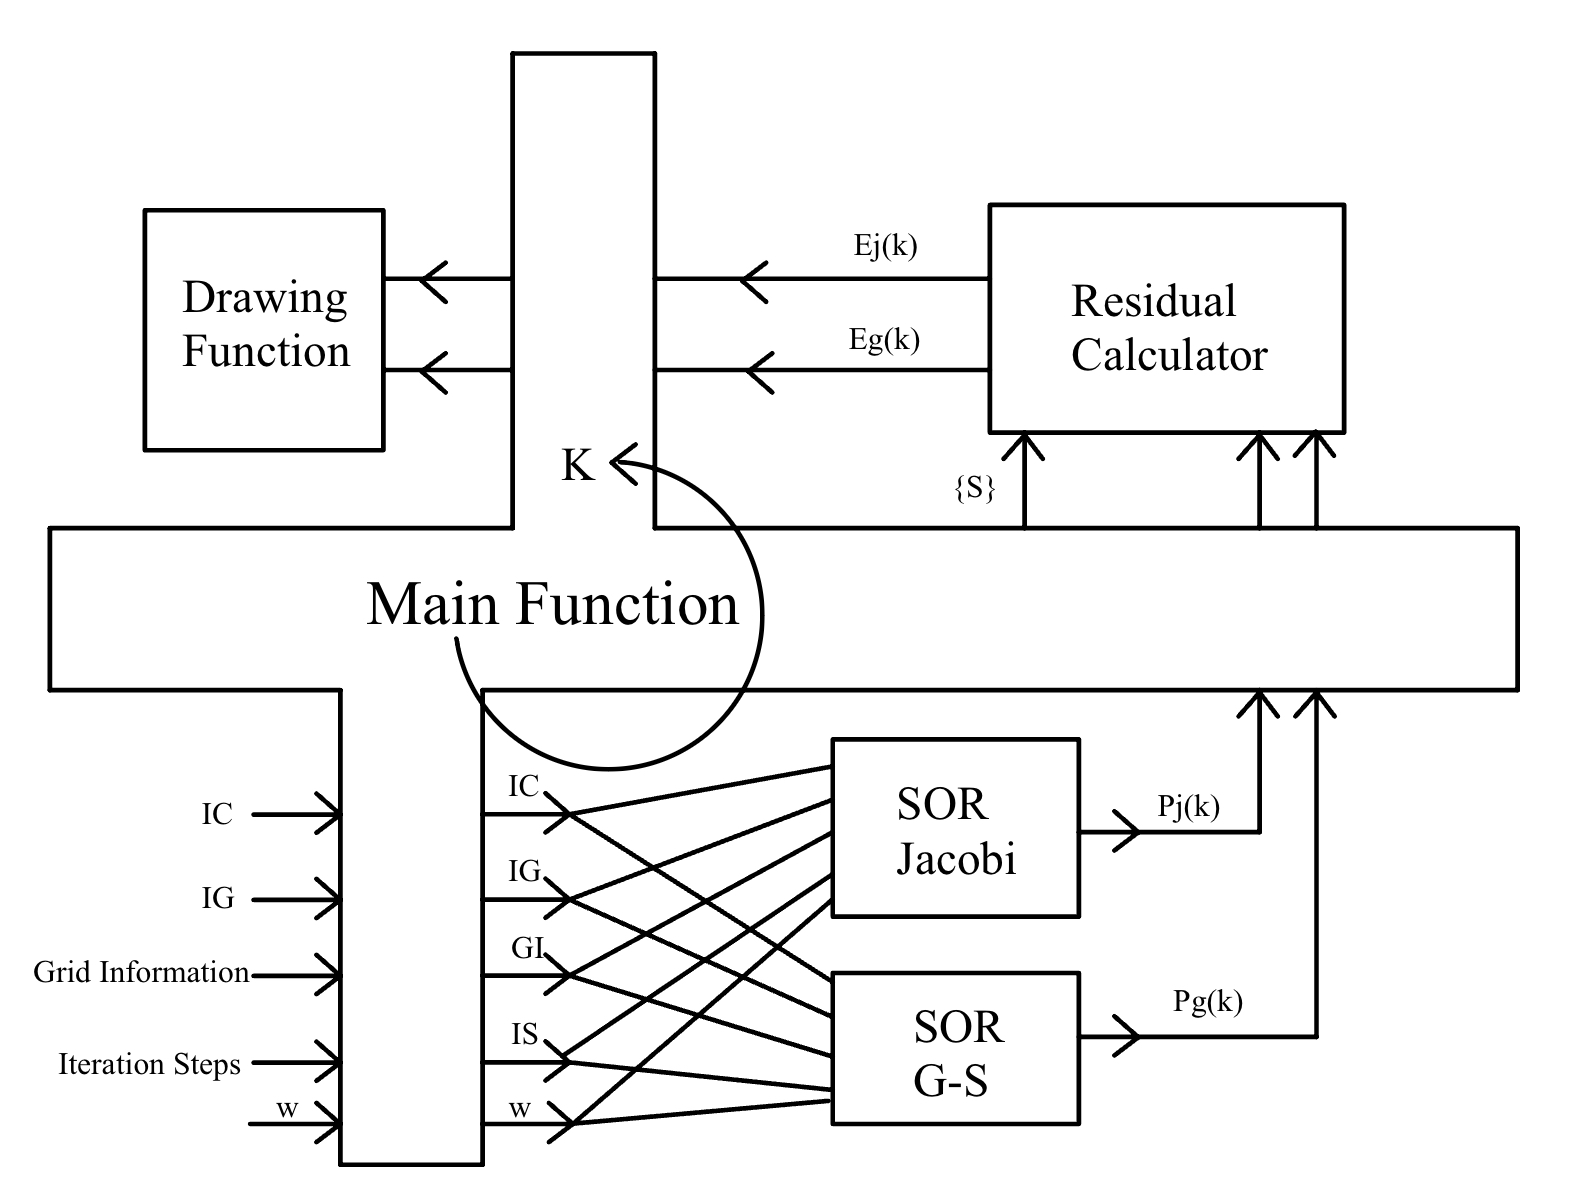
\includegraphics[width=0.6\textwidth]{diagram2.jpg}
    \label{diagram.jpg}
    %\caption{Iteration times as k=200}
\end{figure}






Using w from 0.1 to 2, step size 0.1, initial guess(IG)=0 everywhere,
the result is showing below:



\begin{figure}[H]
    \centering
    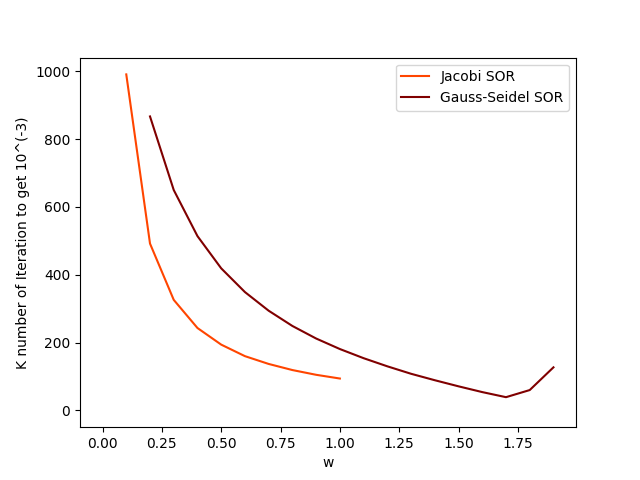
\includegraphics[width=0.8\textwidth]{SOR diagram.png}
    \label{SOR diagram.png}
    %\caption{Iteration times as k=200}
\end{figure}

It could be seen for Jacobi, the most efficient w is still 1, espically,
Overlaxization Jacobi is not work (iteration cannot reduce error in $10^{-3}$) but for 
Gauss-Seidel, the most efficient w is about 1.7 (betweem 1.5 to 1.75 
specifically).

The result for G-S SOR is showing below:\\


w in range [0,1]:

\begin{table}[h]
    \centering
    \begin{tabular}{cccccccccccc}
    \hline
    w & 0.0 & 0.1 & 0.2 & 0.3 & 0.4 & 0.5 & 0.6 & 0.7 & 0.8 & 0.9 & 1.0 \\ \hline
    k & None & None & 867 & 650 & 514 & 419 & 349 & 294 & 249 & 212 & 181 \\ \hline
    \end{tabular}
\end{table}

w in range [1.1,1.9]:
\begin{table}[h]
    \centering
    

    \begin{tabular}{cccccccccc}
    \hline
    w & 1.1 & 1.2 & 1.3 & 1.4 & 1.5 & 1.6 & 1.7 & 1.8 & 1.9 \\ \hline
    k & 154 & 130 & 108 & 89 & 71 & 54 & 39 & 60 & 127 \\ \hline
    \end{tabular}
    \caption{Values of w and k}
\end{table}

It could be found the optimal w is 1.7 in this comparsion (corrosponding
k is 39), where w is the relaxization factor, and k is the iteration 
number each relaxization factor need to let error converge to $10^{-3}$.\\



For other initial guesses, the result is showing below

    
\begin{figure}[H]
    \centering
    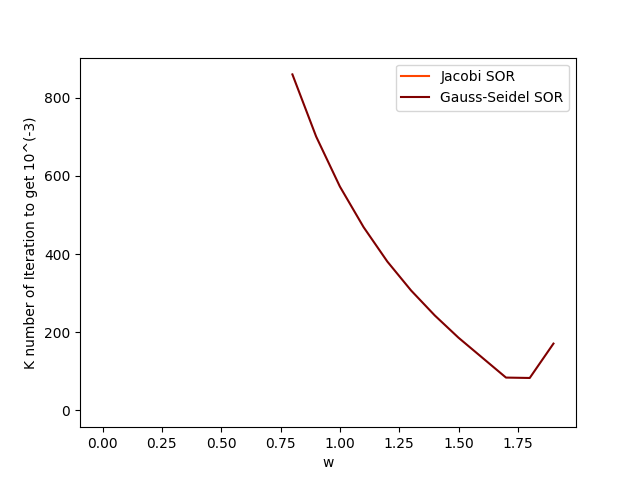
\includegraphics[width=0.45\textwidth]{SORIG2.png}
    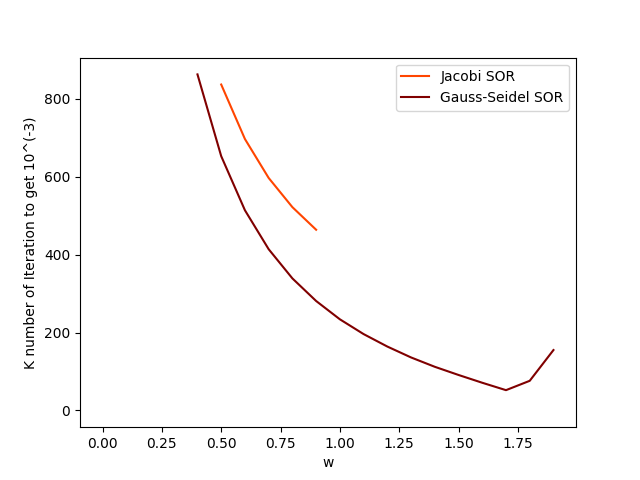
\includegraphics[width=0.45\textwidth]{SORIGR.png}
    \label{SORIG2.png}
    \caption{IG=xiyj(left) result and IG=random(right)result }
\end{figure}


We could also notice in other initial gursses, the optimal relaxization 
w for Gauss-Sediel SOR is also around 1.7. Initial guess is not much
influensional to the optimal relaxization w.





\section{(3) SRJ with two parameter relaxization }


\subsection{Alternative SOR Reach}
For this section, we are using two w to speed up more for different scheme
in different condition. \\

SRJ, which is Scheduled Relaxation Jacobi scheme, could speed up Jacobi
much faster, according to \textit{XiYang and Mittal, 2015}, is using underrelaxation
and overrelaxation generate fast convergence of solution.\\

However, according to the paper, it could been seen the optimal overrelaxation 
parameter is much higher while its show time in iteration in decreasing (amlost 1/100),
for the more simplified iteration, we are going to find parameters between (0,2), 
try to find optimal parameter combinations speed up Jacobi.\\



As w we choose is in range (0,1) for underrelaxation
, and in range (1,2) for overrelaxation, the most simple case come in to
mind is Complementarity w for under and over relaxization, where is using
$w_{1}$ in range (0,1)  and $w_{2}$ in range (1,2), and exchange using
$w_1$ and $w_2$ alternativly each iteration step.\\


Where Alt Fn is an function choosing w in {w} group each steps, using iteration
number t (t in range (0,k)) as choosing parameter.\\

Using iteration times is 100. The result is showing below: 

\begin{figure}[H]
    \centering
    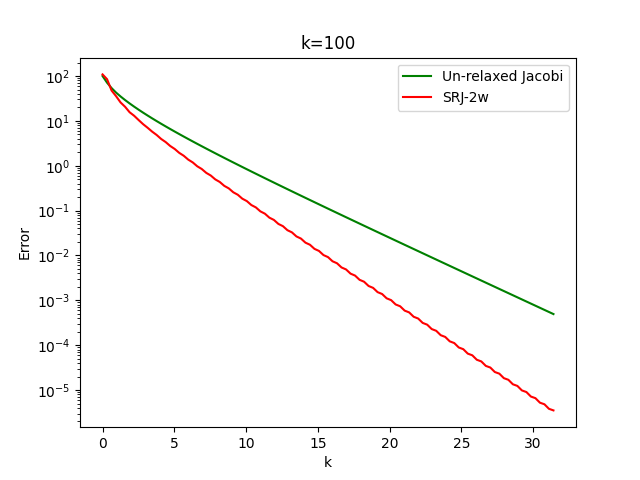
\includegraphics[width=0.7\textwidth]{SRJ1.png    }
    \label{SRJ1.png    }
    %\caption{Iteration times as k=200}
\end{figure}

The optimal combination for alternative w is: $ w_1 = 0.7 $, $ w_2 = 2.0 $,
which result could be observed better than non-relaxed Jacobi.






























\section{(4) SRJ reach for three-parameter optimization}




Using three parameter $(w) = (w1,w2,w3)$, where w1 in range[1,2], w2 in range[1.1,2], 
w3 in range[1,1.1], the result is showing below:


$(w1,w2,w3) = (1.9 , 2 , 0.6)$



\begin{figure}[H]
    \centering
    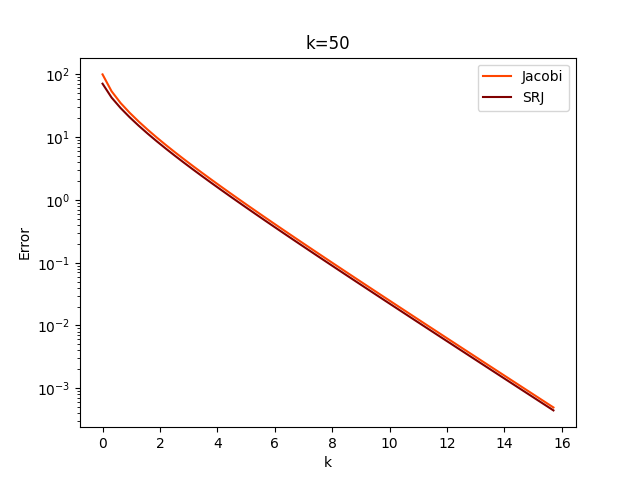
\includegraphics[width=0.7\textwidth]{3SRJ.png   }
    \label{3SRJ.png   }
    %\caption{Iteration times as k=200}
\end{figure}


It could been seen by using three parameters in range (0,2), the Jacobi could been
little bit speed up, as iteration times is not that large and our seeking solution
not need to be extremely accurate.\\

According to \textit{XiYang and Mittal, 2015}, the optimal relaxization parameter
combination is used overrelaxation for only few times durning whole iteration, 
while using the underrelaxation for most of times. Also, it shows the relaxization
order is not that influensional on result, thus we choose w1 as the largest 
iteration parameter only for 1 time, and other two take most of times.\\

Expand our range for parameter in range (0,10), for iteration number k=100,

$(n(w1),n(w2),n(w3))=(1,9,90)$, \\

the optimal combination for w is showing below:

$(w1,w2,w3) = (9.3, 1.1 , 1.0)$,

Use this combination, compare to un-relaxed Jacobi, the result is showing below:



\begin{figure}[H]
    \centering
    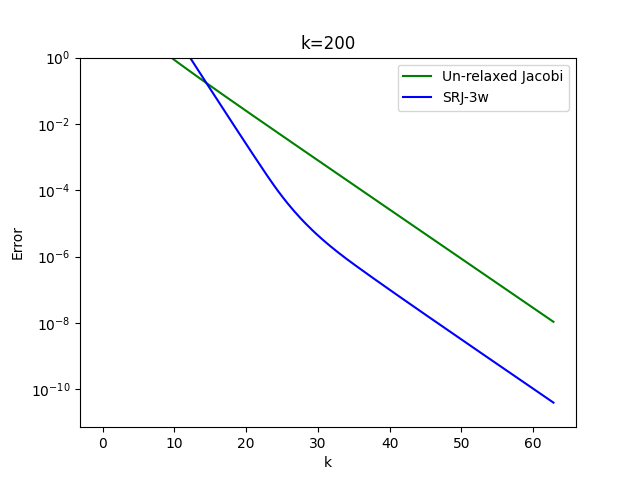
\includegraphics[width=0.7\textwidth]{SRJ9.3_2.1_1.0a.png  }
    \label{SRJ9.3_1.1_2.0.png   }
    %\caption{Iteration times as k=200}
\end{figure}


This diagram's Error is means Error factot,
which means the error of SRJ jacobi divide by error of jacobi
shows by using SRj method from \textit{XiYang and Mittal, 2015}, 
with three parameters, could obviously reduce error of Jacobi.




\subsection{Comparsion-2 Parameters with 3 Parameters(2ws VS 3ws)}

In this section, we are using our 2-parameter's relaxization, which we are using
(0.7,2.0), alternatively, compare with our 3-parameter's relaxization, where 
we re using (9.3,1.1,1.0), frequency(1:9:90), to see if we apply more parameters,
Jacobi method could be much faster.\\



Compare to our 2-parameters shoution, the result is showing below:


\begin{figure}[H]
    \centering
    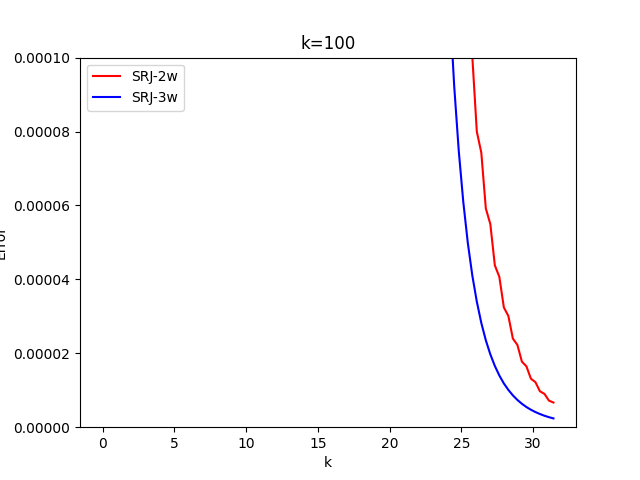
\includegraphics[width=0.7\textwidth]{pcompare1.PNG   }
    
    
    \label{pcompare1.PNG    }
    %\caption{Iteration times as k=200}
\end{figure}

It could find our 3-parameters solution converge much faster than 2-parameters
SRJ solution.


\begin{figure}[H]
    \centering
    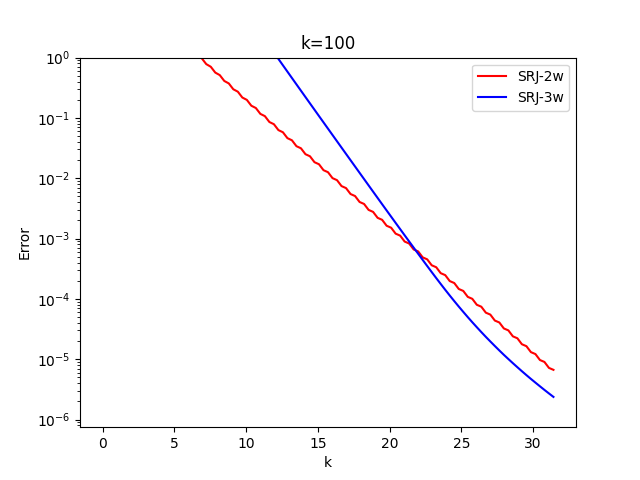
\includegraphics[width=0.7\textwidth]{pcompare2.PNG }
    
    \label{pcompare1.PNG    }
    %\caption{Iteration times as k=200}
\end{figure}

This is the result showing error in log scale, it is much more obvious the 
three-parameter relaxization converge much more faster than 2-parameter relaxization,
and converge as expected.



Compare with un-relaxed Jacobi, the result is showing below:

\begin{figure}[H]
    \centering
    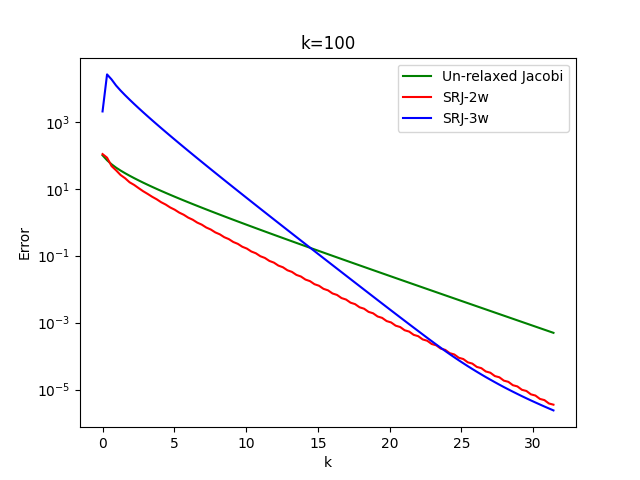
\includegraphics[width=0.7\textwidth]{pcomparetotal.PNG }
    
    \label{pcompare1.PNG    }
    %\caption{Iteration times as k=200}
\end{figure}

It could be seen finally our 3-parameter's relaxization method will make Jacobi
converge faster, which means it will be oppoitunity for Scheduled Relaxization
using more parameters to speed-up Jacobi method.



\section{Conclusion}

In this experiment, we applied Jacobi method with Gauss-Seidel method in grid to 
solve 2-D Laplace Equation, built algorithms for solver, and experimented SOR method,
Scheduled Relaxization method to speed up our old solver.\\

It could be shown that for more general condition, Gauss-Seidel converge faster than
Jacobi, while Jacobi only have small middle wavenumber range faster than G-S.\\

For SOR method, only SOR G-S have better converge performance, which using w around
1.7.\\

For Scheduled Relaxization, using 2-parameter and 3-parameter could speed up Jacobi
method. For 2-parameters, we use alternative relaxization for w=(0.7,2.0), 
frequency (1:1). And for 3-parameters, we use w=(9.3,1.1,1.0), frequency(1:9:90), 
which can finally get fastest convergence result than 2-parameter method and un-relaxed
Jacobi.









%%%%%%%%%%%%%%%%%%%%%%%%%%%%%%%%%%%%%%%%%%%%%%%%%%%%%%%%%%%%%%%
%%%%%%%%%%%%%%%%%%%%%%%%%%%%%%%%%%%%%%%%%%%%%%%%%%%%%%%%%%%%%%%
%%%%%%%%%%%%%%%%%%%%%%%%%%%%%%%%%%%%%%%%%%%%%%%%%%%%%%%%%%%%%%%
\newpage
\section*{Appendix}
% 在目录中添加Appendix
\addcontentsline{toc}{section}{Appendix}
\begin{scriptsize}
\begin{lstlisting}[language=python,caption={(1)-The python Source code of Algorithm}]


    import copy #for Python, need copy op to avoid 

    def Jacobi(P_input, x_len, y_len): #Jacobi method Pin-->Pout
        P_old = copy.deepcopy(P_input)
        P_new = copy.deepcopy(P_input)
        for j in range(1,y_len-1):
            for i in range(1,x_len-1): 
                P_new[j][i] = \
                    1/4 * (  P_old[j][i-1] + P_old[j][i+1] + P_old[j-1][i] + P_old[j+1][i] )
        return P_new
    
    def GS(P_input, x_len, y_len): #Gauss Sadiel method Pin-->Pout
        Pg = copy.deepcopy(P_input)
        for j in range(1,y_len-1):
            for i in range(1,x_len-1): 
                Pg[j][i] = \
                    1/4 * (  Pg[j][i-1] + Pg[j][i+1] + Pg[j-1][i] + Pg[j+1][i] )
        return Pg
    
    
    def Res(r,Pin,d,x_len,y_len): #calcuate residual (Pin, source)-->Rout
        P = copy.deepcopy(Pin)
        rc = copy.deepcopy(r)
        for j in range(1,y_len-1):
            for i in range(1,x_len-1): 
                rc[j][i] = \
                    ( P[j][i-1] + P[j][i+1] + P[j-1][i] + P[j+1][i] - 4*P[j][i] )/(d**2)
        return rc
    
    def Error(r_in, x_len, y_len): #calculate error Rin-->e out
        r = copy.deepcopy(r_in)
        e = 0
        for j in range(1,y_len-1):
            for i in range(1,x_len-1): 
                e += abs(r[j][i])
        return e
    
    
    import matplotlib.pyplot as plt
    import numpy as np
    import matplotlib as mpl
    
    def eploting(  ej, egs,   d,  x_len, y_len,   k     ):
        x = [0 for _ in range(0, k+1)]
        for c in range(0,k+1):
            x[c] = c*d
        plt.plot(x, ej, color = 'blue', label = 'Jacobi')
        plt.plot(x, egs, color = 'red', label = 'Gauss-Seidel')
        plt.show()
    
    
    
    
    ########################## main function below ########
    
    
    def main():
        import math
    
    
        #import grid data
        pi = math.pi
        x_max = 2*pi
        y_max = 2*pi
        d = 2*pi/20
        dx = dy = d
        x_len = int(x_max/dx+1)
        y_len = int(y_max/dy+1)
    
        # x_len: the number of x points
        # the first x point is x[0], the last x point is x[x_len -1]
    
        k = 50
    
        #import Boundary Condition (BC)
        P = [[0 for _ in range(0,x_len+1)] for _ in range(0, y_len+1)]
    
        for i in range(0,x_len):
            sin = math.sin
            P[0][i] = sin(2*i*dx) + sin(5*i*dx) + sin(7*i*dx)
            P[y_len-1][i] = 0
        for j in range(0,y_len):
            P[j][0] = 0
            P[j][x_len-1] = 0
    
        #import Initial Guess (IG)
        IG = 0 #change IG for different guess
        for j in range(1,y_len-1):
            for i in range(1,x_len-1):
                P[j][i] = IG
        
        #P_input = copy.deepcopy(P)
        r = copy.deepcopy(P)
        e = [0 for _ in range(0,k+1)]
        ej = copy.deepcopy(e)
        egs = copy.deepcopy(e)
    
        P_Jin = copy.deepcopy(P)
        P_GSin = copy.deepcopy(P)
        
    
        for t in range(0,k+1):
            
            P_Jacobi = Jacobi(P_Jin, x_len, y_len)
            P_GS = GS(P_GSin, x_len, y_len)
    
            P_Jin = P_Jacobi
            P_GSin = P_GS
    
            r_J = Res(r,P_Jacobi,d,x_len,y_len)
            r_GS = Res(r,P_GS,d,x_len,y_len)
            ej[t] = Error(r_J, x_len, y_len)
            egs[t] = Error(r_GS, x_len, y_len)
        
        
        #print(1)
        #P_Jacobi = Jacobi(P_Jin, x_len, y_len)
    
        #print(P_input)
        #print(P_Jacobi)
        eploting(  ej, egs,  d,   x_len, y_len,     k   )
        #print(ej)
    
    
    
    
    
    
    # main function operator
    if __name__ == "__main__":
        main()
    
    
    
    
    
    
\end{lstlisting}
\end{scriptsize}


%%%%%%%%%%%%%%%%%%%%%%%%%%%%%%%%%%%%%%%%%%%%%%%%%%%%%%%%%%%%%%%


\begin{scriptsize}
    \begin{lstlisting}[language=python,caption={(2)(IG=0)-The python Source code of Algorithm}]
    
    
import copy #for Python, need copy op to avoid 

def Jacobi(P_input, x_len, y_len): #Jacobi method Pin-->Pout
    P_old = copy.deepcopy(P_input)
    P_new = copy.deepcopy(P_input)
    for j in range(1,y_len-1):
        for i in range(1,x_len-1): 
            P_new[j][i] = \
                1/4 * (  P_old[j][i-1] + P_old[j][i+1] + P_old[j-1][i] + P_old[j+1][i] )
    return P_new




def GS(P_input, x_len, y_len): #Gauss Sadiel method Pin-->Pout
    Pg = copy.deepcopy(P_input)
    for j in range(1,y_len-1):
        for i in range(1,x_len-1): 
            Pg[j][i] = \
                1/4 * (  Pg[j][i-1] + P_input[j][i+1] + Pg[j-1][i] + P_input[j+1][i] )
    return Pg



def SORJacobi(P_inputSOR, x_len, y_len, w): #Jacobi SOR method Pin-->Pout
    P_oldSOR = copy.deepcopy(P_inputSOR)
    P_newSOR = copy.deepcopy(P_inputSOR)
    for j in range(1,y_len-1):
        for i in range(1,x_len-1): 
            P_newSOR[j][i] = \
                1/4 * (  P_oldSOR[j][i-1] + P_oldSOR[j][i+1] + P_oldSOR[j-1][i] + P_oldSOR[j+1][i] ) *w + (1-w)*P_oldSOR[j][i]
    return P_newSOR


def SORGS(P_inputSOR, x_len, y_len,w): #Gauss Sadiel SOR method Pin-->Pout
    PgSOR = copy.deepcopy(P_inputSOR)
    for j in range(1,y_len-1):
        for i in range(1,x_len-1): 
            PgSOR[j][i] = \
                1/4 * (  PgSOR[j][i-1] + P_inputSOR[j][i+1] + PgSOR[j-1][i] + P_inputSOR[j+1][i] )*w + (1-w)*P_inputSOR[j][i]
    return PgSOR





def Res(r,Pin,d,x_len,y_len): #calcuate residual (Pin, source)-->Rout
    P = copy.deepcopy(Pin)
    rc = copy.deepcopy(r)
    for j in range(1,y_len-1):
        for i in range(1,x_len-1): 
            rc[j][i] = \
                ( P[j][i-1] + P[j][i+1] + P[j-1][i] + P[j+1][i] - 4*P[j][i] )/(d**2)
    return rc

def Error(r_in, x_len, y_len): #calculate error Rin-->e out
    r = copy.deepcopy(r_in)
    e = 0
    for j in range(1,y_len-1):
        for i in range(1,x_len-1): 
            e += abs(r[j][i])
    return e


import matplotlib.pyplot as plt
#import numpy as np
import matplotlib as mpl

def nploting(  nj, ngs ):
    w = [0 for _ in range(0, 20)]
    for c in range(1,20):
        w[c] = c*0.1
    
    plt.plot(w, nj, color = 'orangered', label = 'Jacobi SOR')
    plt.plot(w, ngs, color = 'maroon', label = 'Gauss-Seidel SOR')

    plt.legend()
    plt.xlabel('w')
    plt.ylabel('K number of Iteration to get 10^(-3)')
    #plt.ylim(0,5)
    #plt.ylim(0,10**(-10))





    plt.show()




########################## main function below ########


def main():
    import math


    #import grid data
    pi = math.pi
    x_max = 2*pi
    y_max = 2*pi
    d = 2*pi/20
    dx = dy = d
    x_len = int(x_max/dx+1)
    y_len = int(y_max/dy+1)

    # x_len: the number of x points
    # the first x point is x[0], the last x point is x[x_len -1]

    k = 1000

    #import Boundary Condition (BC)
    P = [[0 for _ in range(0,x_len+1)] for _ in range(0, y_len+1)]

    for i in range(0,x_len):
        sin = math.sin
        P[0][i] = sin(2*i*dx) + sin(5*i*dx) + sin(7*i*dx)
        P[y_len-1][i] = 0
    for j in range(0,y_len):
        P[j][0] = 0
        P[j][x_len-1] = 0

    #import Initial Guess (IG)
    IG = 0 #change IG for different guess
    for j in range(1,y_len-1):
        for i in range(1,x_len-1):
            P[j][i] = IG
    
    #P_input = copy.deepcopy(P)
    r = copy.deepcopy(P)
    e = [0 for _ in range(0,k+1)]
    ej = copy.deepcopy(e)
    egs = copy.deepcopy(e)

    P_Jin = copy.deepcopy(P)
    P_GSin = copy.deepcopy(P)


    en = 10**(-3)

    #calculate iteration number of Jacobi
    for t in range(0,k+1):
        
        P_Jacobi = Jacobi(P_Jin, x_len, y_len)

        P_Jin = P_Jacobi

        r_J = Res(r,P_Jacobi,d,x_len,y_len)
 
        ej = Error(r_J, x_len, y_len)

        if ej <= en:
            nj = t
            break
        if t == k:
            nj= 200
    
    #calculate interation number of Gauss-Seidel
    for t in range(0,k+1):
        
        P_GS = GS(P_GSin, x_len, y_len)

        P_GSin = P_GS


        r_GS = Res(r,P_GS,d,x_len,y_len)

        egs = Error(r_GS, x_len, y_len)
        if egs <= en:
            ngs = t
            break
        if t == k:
            ngs = 200

    #calculate iteration times of different w
    nj = [0 for _ in range(0,20)]
    ngs = [0 for _ in range(0,20)]

    for wc in range(1,20):
        w = wc*0.1
        r = copy.deepcopy(P)

        P_Jin = copy.deepcopy(P)
        P_GSin = copy.deepcopy(P)


        for t in range(0,k+1):
            
            
            SORP_Jacobi = SORJacobi(P_Jin, x_len, y_len, w)

            P_Jin = SORP_Jacobi

            SORr_J = Res(r,SORP_Jacobi,d,x_len,y_len)

            SORej = Error(SORr_J, x_len, y_len)
            if SORej <=en:
                nj[wc] = t
                break
            if t == k:
                nj[wc] = None
        
        for t in range(0,k+1):
            
            
            SORP_GS = SORGS(P_GSin, x_len, y_len, w)

            P_GSin = SORP_GS

            SORr_GS = Res(r,SORP_GS,d,x_len,y_len)

            SORegs = Error(SORr_GS, x_len, y_len)
            if SORegs <=en:
                ngs[wc] = t
                break
            if t == k:
                ngs[wc] = None


   
    #nploting( nj , ngs)
    print(SORegs)
    
    #print(ej)






# main function operator
if __name__ == "__main__":
    main()










\end{lstlisting}
\end{scriptsize}


%%%%%%%%%%%%%%%%%%%%%%%%%%%%%%%%%%%%%%%%%%%%%%%%%%%%%%%%%%%%%%%


\begin{scriptsize}
    \begin{lstlisting}[language=python,caption={(3)-The python Source code}]

import copy #for Python, need copy op to avoid 

def Jacobi(P_input, x_len, y_len): #Jacobi method Pin-->Pout
    P_old = copy.deepcopy(P_input)
    P_new = copy.deepcopy(P_input)
    for j in range(1,y_len-1):
        for i in range(1,x_len-1): 
            P_new[j][i] = \
                1/4 * (  P_old[j][i-1] + P_old[j][i+1] + P_old[j-1][i] + P_old[j+1][i] )
    return P_new




def GS(P_input, x_len, y_len): #Gauss Sadiel method Pin-->Pout
    Pg = copy.deepcopy(P_input)
    for j in range(1,y_len-1):
        for i in range(1,x_len-1): 
            Pg[j][i] = \
                1/4 * (  Pg[j][i-1] + P_input[j][i+1] + Pg[j-1][i] + P_input[j+1][i] )
    return Pg



def SORJacobi(P_inputSOR, x_len, y_len, w): #Jacobi SOR method Pin-->Pout
    P_oldSOR = copy.deepcopy(P_inputSOR)
    P_newSOR = copy.deepcopy(P_inputSOR)
    for j in range(1,y_len-1):
        for i in range(1,x_len-1): 
            P_newSOR[j][i] = \
                1/4 * (  P_oldSOR[j][i-1] + P_oldSOR[j][i+1] + P_oldSOR[j-1][i] + P_oldSOR[j+1][i] ) *w + (1-w)*P_oldSOR[j][i]
    return P_newSOR


def SORGS(P_inputSOR, x_len, y_len,w): #Gauss Sadiel SOR method Pin-->Pout
    PgSOR = copy.deepcopy(P_inputSOR)
    for j in range(1,y_len-1):
        for i in range(1,x_len-1): 
            PgSOR[j][i] = \
                1/4 * (  PgSOR[j][i-1] + P_inputSOR[j][i+1] + PgSOR[j-1][i] + P_inputSOR[j+1][i] )*w + (1-w)*P_inputSOR[j][i]
    return PgSOR





def Res(r,Pin,d,x_len,y_len): #calcuate residual (Pin, source)-->Rout
    P = copy.deepcopy(Pin)
    rc = copy.deepcopy(r)
    for j in range(1,y_len-1):
        for i in range(1,x_len-1): 
            rc[j][i] = \
                ( P[j][i-1] + P[j][i+1] + P[j-1][i] + P[j+1][i] - 4*P[j][i] )/(d**2)
    return rc

def Error(r_in, x_len, y_len): #calculate error Rin-->e out
    r = copy.deepcopy(r_in)
    e = 0
    for j in range(1,y_len-1):
        for i in range(1,x_len-1): 
            e += abs(r[j][i])
    return e


import matplotlib.pyplot as plt
#import numpy as np
import matplotlib as mpl

def eploting(   ej, eSORj,    d,    k     ):
    x = [0 for _ in range(0, k+1)]
    for c in range(0,k+1):
        x[c] = c*d
    plt.plot(x, ej, color = 'orangered', label = 'Jacobi')
    plt.plot(x, eSORj, color = 'maroon', label = 'SRJ')
    plt.legend()

    #plt.yscale('log')
    plt.xlabel('k')
    plt.ylabel('Error')
    #plt.ylim(0,1)
    plt.ylim(0,10**(-2))

    plt.title("k=%d"%k)





    plt.show()




def altw(w1,w2,k):
    wlist = [w1,w2]
    wselect = wlist[k%len(wlist)]
    return wselect
    




########################## main function below ########
########################## main function below ########
########################## main function below ########
########################## main function below ########


def main():
    import math

    ########################## Grid Information v ######
    ########################## Grid Information v ######
    
    #import grid data
    pi = math.pi
    x_max = 2*pi
    y_max = 2*pi
    d = 2*pi/20
    dx = dy = d
    x_len = int(x_max/dx+1)
    y_len = int(y_max/dy+1)

    # x_len: the number of x points
    # the first x point is x[0], the last x point is x[x_len -1]

    k = 1000

    #import Boundary Condition (BC)
    P = [[0 for _ in range(0,x_len+1)] for _ in range(0, y_len+1)]

    for i in range(0,x_len):
        sin = math.sin
        P[0][i] = sin(2*i*dx) + sin(5*i*dx) + sin(7*i*dx)
        P[y_len-1][i] = 0
    for j in range(0,y_len):
        P[j][0] = 0
        P[j][x_len-1] = 0
    
    ########################## Grid Information ^ ######



    #import Initial Guess (IG)
    IG = 0 #change IG for different guess
    for j in range(1,y_len-1):
        for i in range(1,x_len-1):
            P[j][i] = IG
    
    #P_input = copy.deepcopy(P)
    r = copy.deepcopy(P)
    e = [0 for _ in range(0,k+1)]
    ej = copy.deepcopy(e)
    egs = copy.deepcopy(e)

    P_Jin = copy.deepcopy(P)
    P_GSin = copy.deepcopy(P)


    #en = 10**(-3)
    en = 1


    #calculate iteration times of different w

    w1o = 0
    w2o = 0
    ko = 0
    SORejo = 0



    for w1 in range(1,11):
        w1 = w1*0.1
        for w2 in range(11,101):
            w2 = w2*0.1

            r = copy.deepcopy(P)

            P_Jin = copy.deepcopy(P)
            P_GSin = copy.deepcopy(P)

            for t in range(0,k+1):

                w = altw(w1,w2,t)
                 
                SORP_Jacobi = SORJacobi(P_Jin, x_len, y_len, w)

                P_Jin = SORP_Jacobi

            SORr_J = Res(r,SORP_Jacobi,d,x_len,y_len)

            SORej = Error(SORr_J, x_len, y_len)

            if SORej <=en:
                en = SORej
                w1o = w1
                w2o = w2
                ko = k  
                SORejo = SORej


    print(w1o)
    print(w2o)
    print(ko)
    
    #P_input = copy.deepcopy(P)
    r = copy.deepcopy(P)
    e = [0 for _ in range(0,k+1)]
    ej = copy.deepcopy(e)

    P_Jin = copy.deepcopy(P)    
    P_Jin1 = copy.deepcopy(P)  

    eSORj = copy.deepcopy(e)

    for t in range(0,k+1):
        
        P_Jacobi = Jacobi(P_Jin, x_len, y_len)

        P_Jin = P_Jacobi

        r_J = Res(r,P_Jacobi,d,x_len,y_len)

        ej[t] = Error(r_J, x_len, y_len)
        
        ################# Plot SRJ w1=0.6 w2=1.1 #################
        
        w = altw(w1,w2,k) # Alt fn. odd iteration doing w1, even iteration doing w2
                 
        SORP_Jacobi = SORJacobi(P_Jin1, x_len, y_len, w)

        P_Jin1 = SORP_Jacobi

        SORr_J = Res(r,SORP_Jacobi,d,x_len,y_len)

        eSORj[t] = Error(SORr_J, x_len, y_len)

    print(eSORj[k]/ej[k])
    print(w)
    
    eploting(   ej, eSORj,    d,    k     )





# main function operator
if __name__ == "__main__":
    main()








    


\end{lstlisting}
\end{scriptsize}

%%%%%%%%%%%%%%%%%%%%%%%%%%%%%%%%%%%%%%%%%%%%%%%%%%%%%%%%%%%%%%%


\begin{scriptsize}
    \begin{lstlisting}[language=python,caption={(4)-The python Source code}]

import copy #for Python, need copy op to avoid 

def Jacobi(P_input, x_len, y_len): #Jacobi method Pin-->Pout
    P_old = copy.deepcopy(P_input)
    P_new = copy.deepcopy(P_input)
    for j in range(1,y_len-1):
        for i in range(1,x_len-1): 
            P_new[j][i] = \
                1/4 * (  P_old[j][i-1] + P_old[j][i+1] + P_old[j-1][i] + P_old[j+1][i] )
    return P_new




def GS(P_input, x_len, y_len): #Gauss Sadiel method Pin-->Pout
    Pg = copy.deepcopy(P_input)
    for j in range(1,y_len-1):
        for i in range(1,x_len-1): 
            Pg[j][i] = \
                1/4 * (  Pg[j][i-1] + P_input[j][i+1] + Pg[j-1][i] + P_input[j+1][i] )
    return Pg



def SORJacobi(P_inputSOR, x_len, y_len, w): #Jacobi SOR method Pin-->Pout
    P_oldSOR = copy.deepcopy(P_inputSOR)
    P_newSOR = copy.deepcopy(P_inputSOR)
    for j in range(1,y_len-1):
        for i in range(1,x_len-1): 
            P_newSOR[j][i] = \
                1/4 * (  P_oldSOR[j][i-1] + P_oldSOR[j][i+1] + P_oldSOR[j-1][i] + P_oldSOR[j+1][i] ) *w + (1-w)*P_oldSOR[j][i]
    return P_newSOR


def SORGS(P_inputSOR, x_len, y_len,w): #Gauss Sadiel SOR method Pin-->Pout
    PgSOR = copy.deepcopy(P_inputSOR)
    for j in range(1,y_len-1):
        for i in range(1,x_len-1): 
            PgSOR[j][i] = \
                1/4 * (  PgSOR[j][i-1] + P_inputSOR[j][i+1] + PgSOR[j-1][i] + P_inputSOR[j+1][i] )*w + (1-w)*P_inputSOR[j][i]
    return PgSOR





def Res(r,Pin,d,x_len,y_len): #calcuate residual (Pin, source)-->Rout
    P = copy.deepcopy(Pin)
    rc = copy.deepcopy(r)
    for j in range(1,y_len-1):
        for i in range(1,x_len-1): 
            rc[j][i] = \
                ( P[j][i-1] + P[j][i+1] + P[j-1][i] + P[j+1][i] - 4*P[j][i] )/(d**2)
    return rc

def Error(r_in, x_len, y_len): #calculate error Rin-->e out
    r = copy.deepcopy(r_in)
    e = 0
    for j in range(1,y_len-1):
        for i in range(1,x_len-1): 
            e += abs(r[j][i])
    return e


import matplotlib.pyplot as plt
#import numpy as np
import matplotlib as mpl

def eploting(   ej, eSORj,    d,    k     ):
    x = [0 for _ in range(0, k+1)]
    for c in range(0,k+1):
        x[c] = c*d
    
    f = [0 for _ in range(0,k+1)]

    for t in range(0,k+1):
        f[t] = eSORj[t]/ej[t]
    '''
    plt.plot(x, ej, color = 'orangered', label = 'Jacobi')
    plt.plot(x, eSORj, color = 'maroon', label = 'SRJ')
    '''
    plt.plot(x, f, color = 'maroon', label = 'factor with Jacobi')


    plt.legend()

    #plt.yscale('log')
    plt.xlabel('k')
    plt.ylabel('Error')
    plt.ylim(0,1)
    #plt.ylim(0,10**(-2))

    plt.title("k=%d"%k)





    plt.show()



def wlist0(w1,w2,w3,k):
    wlist = [w3 for _ in range(0,k+1)]

    for s in range(0,2):
        wlist[s] = w1
    for s in range(2,3):
        wlist[s] = w2

    return wlist



'''

def altw(w1,w2,w3,k):
    # wlist = [w1,w2,w3]

    wlist = wlist0(w1,w2,w3,k)
    wselect = wlist[k]
    
    return wselect
'''




########################## main function below ########
########################## main function below ########
########################## main function below ########
########################## main function below ########




def main():
    import math


    from tqdm import tqdm
    

    ########################## Grid Information v ######
    ########################## Grid Information v ######
    
    #import grid data
    pi = math.pi
    x_max = 2*pi
    y_max = 2*pi
    d = 2*pi/20
    dx = dy = d
    x_len = int(x_max/dx+1)
    y_len = int(y_max/dy+1)

    # x_len: the number of x points
    # the first x point is x[0], the last x point is x[x_len -1]

    k = 100

    #import Boundary Condition (BC)
    P = [[0 for _ in range(0,x_len+1)] for _ in range(0, y_len+1)]

    for i in range(0,x_len):
        sin = math.sin
        P[0][i] = sin(2*i*dx) + sin(5*i*dx) + sin(7*i*dx)
        P[y_len-1][i] = 0
    for j in range(0,y_len):
        P[j][0] = 0
        P[j][x_len-1] = 0
    
    ########################## Grid Information ^ ######



    #import Initial Guess (IG)
    IG = 0 #change IG for different guess
    for j in range(1,y_len-1):
        for i in range(1,x_len-1):
            P[j][i] = IG
    
    #P_input = copy.deepcopy(P)
    r = copy.deepcopy(P)
    e = [0 for _ in range(0,k+1)]
    ej = copy.deepcopy(e)
    egs = copy.deepcopy(e)

    P_Jin = copy.deepcopy(P)
    P_GSin = copy.deepcopy(P)


    #en = 10**(-3)
    en = 1


    #calculate iteration times of different w

    w1o = 0
    w2o = 0
    ko = 0
    SORejo = 0



    for w1 in tqdm(range(1,1001),desc='total calculation'):
        w1 = w1*0.1
        for w2 in range(11,21):
            w2 = w2*0.1
            for w3 in range(1,21):
                w3 = w3*0.1

                for t in range(0,k+1):

                    w = wlist0(w1,w2,w3,k)[t]
                    
                    SORP_Jacobi = SORJacobi(P_Jin, x_len, y_len, w)

                    P_Jin = SORP_Jacobi

                SORr_J = Res(r,SORP_Jacobi,d,x_len,y_len)

                SORej = Error(SORr_J, x_len, y_len)

                if SORej <=en:
                    en = SORej
                    w1o = w1
                    w2o = w2
                    w3o = w3
                    ko = k  
                    SORejo = SORej


    print(w1o)
    print(w2o)
    print(w3o)
    print("efefefeffefe")
    print(ko)
    
    #P_input = copy.deepcopy(P)
    r = copy.deepcopy(P)
    e = [0 for _ in range(0,k+1)]
    ej = copy.deepcopy(e)

    P_Jin = copy.deepcopy(P)    

    eSORj = copy.deepcopy(e)

    for t in tqdm(range (0,k+1), desc='final plloting'):
        
        P_Jacobi = Jacobi(P_Jin, x_len, y_len)

        P_Jin = P_Jacobi

        r_J = Res(r,P_Jacobi,d,x_len,y_len)

        ej[t] = Error(r_J, x_len, y_len)
        
        ################# Plot SRJ w1=0.6 w2=1.1 #################
        
        w = wlist0(w1o,w2o,w3o,k)[t] # Alt fn. odd iteration doing w1, even iteration doing w2
                 
        SORP_Jacobi = SORJacobi(P_Jin, x_len, y_len, w)

        P_Jin = SORP_Jacobi

        SORr_J = Res(r,SORP_Jacobi,d,x_len,y_len)

        eSORj[t] = Error(SORr_J, x_len, y_len)

    print(eSORj[k-1]/ej[k-1])
    print(w)
    
    eploting(   ej, eSORj,    d,    k     )





# main function operator
if __name__ == "__main__":
    main()







\end{lstlisting}
\end{scriptsize}



%%%%%%%%%%%%%%%%%%%%%%%%%%%%%%%%%%%%%%%%%%%%%%%%%%%%%%%%%%%%%%%
%%%%%%%%%%%%%%%%%%%%%%%%%%%%%%%%%%%%%%%%%%%%%%%%%%%%%%%%%%%%%%%
%%%%%%%%%%%%%%%%%%%%%%%%%%%%%%%%%%%%%%%%%%%%%%%%%%%%%%%%%%%%%%%



\end{document}